\documentclass[11pt, letterpaper]{report}
\usepackage{amsmath,fullpage,graphicx,amssymb}

\setlength{\parindent}{0em}

\newcommand{\nott}{{\sim}}

\newcommand{\Z}{\mathbb{Z}}
\newcommand{\R}{\mathbb{R}}

\newcommand{\powerset}[1]{\mathcal P \left({#1}\right)}

\begin{document}

{\textbf{Discrete Structures, Fall 2017, Homework 11 Solutions}}

\vspace*{.1in}

You must write the solutions to these problems legibly on your own paper, with
the problems in sequential order, and with all sheets stapled together.

\medskip

\emph{Helpful hint --- read sections 9.1, 9.2, and 9.3 first!}

\medskip

\textbf{For any problem that requires a numerical answer (as opposed to a proof or something written in words), unless otherwise specified, you do not need to fully reduce your
answer to a single number --- you may leave it in a form that uses addition, subtraction, multiplication, division, permutations (i.e., $P(n,k)$ notation)
and combinations (i.e., $\binom{n}{k}$ notation).}

\medskip

\textbf{Show your work for these problems! If you make a calculation error, it is easier to give partial credit if you illustrate how you derived your answer.}





\begin{enumerate}



\item There have been three computer science talks this semester (Slingshot, FedEx, and the industry panel).  Suppose you 
chose at random whether to attend each talk (in other words, for each talk, there is a 50--50 chance that you attended).  Let the letter ``Y''
mean you attended a talk, and ``N'' mean you didn't attend.  So you can encode your attendance at each talk by a 3-character
string of of Ys and/or Ns.  For example, YNN means you attended the Slingshot talk, but not the FedEx or industry
panel talks.  

\begin{enumerate}
        \item List the eight elements in the sample space whose outcomes are all possible ways you could have attended/not 
        attended the talks. 
        
        \textbf{Answer:} $\{YYY,YYN,YNY,YNN,NYY,NYN,NNY,NNN\}$.
        
        \item Write each of these events as a set \emph{and}
find its probability \emph{(reduce each probability to a fraction in lowest terms)}: 
        
        Event X = The event that you attended exactly one of the talks. 
        
        \textbf{Answer:} $X = \{YNN, NYN, NNY\}$.  $P(X) = 3/8$.
        
        Event Y = The event that you attended at least two of the talks.
                
        \textbf{Answer:} $Y = \{YYN, NYY, YNY, YYY\}$.  $P(Y) = 4/8=1/2$.
        
        Event Z = The event that you attended none of the talks.
                
        \textbf{Answer:} $X = \{NNN\}$.  $P(Z) = 1/8$.
        
\end{enumerate}
        
\item \emph{(For this question, reduce each answer to a single integer or to a fraction in lowest terms.)}\begin{enumerate} 
 \item How many positive 3-digit numbers are multiples of 6? 
 
 \textbf{Answer:}  The smallest 3-digit multiple of 6 is 102.  The largest is 996.  $102/6=17$.  $996/6=166$.  $166-17+1=150$.
 
 \item What is the probability that a randomly chosen positive
three-digit integer is a multiple of 6? 

\textbf{Answer:} There are $999-100+1=900$ total 3-digit numbers.  Probability = $150/900$.

\item What is the probability that a randomly chosen positive three-digit integer is a multiple of 7?

\textbf{Answer:} Repeating the process above: 
 The smallest 3-digit multiple of 6 is 105.  The largest is 994.  $105/7=15$.  $994/7=142$.  $142-15+1=128$.  Probability = $128/900$.

\end{enumerate}

\item Suppose that in a certain state, all automobile license plates have four uppercase letters followed by three digits.
\begin{enumerate}
        \item How many different license plates are possible?  
        
        \textbf{Answer:} $26^4 \cdot 10^3$.
        
        \item How many license plates could begin with A and end in 0? 
        
        \textbf{Answer: } In this case there is only one way to perform step 1 (because the first letter must be an A) and only one way to perform step 7 (because the last digit must be a 0). Therefore, the number of license plates is $26\cdot 26 \cdot 26 \cdot 10 \cdot 10 = 17,576,000$.
        
        \item How many license plates could begin with ``TGIF''?
        
        \textbf{Answer: } There's only one way to pick TGIF for the four letter spots, so there are $10 \cdot 10 \cdot 10=1000$ total license plates that start with TGIF.
        
        \item How many license plates are possible in which all the letters and digits are distinct?
        
        \textbf{Answer: }
        
        In this case there are 26 ways to perform step 1, 25 ways to perform step 2, 24 ways to perform step 3, 10 ways to perform step 4, 9 ways to perform step 5, and 8 ways to perform step 6, so the number of license plates is $26 \cdot 25  \cdot 24  \cdot 23  \cdot 10  \cdot 9  \cdot 8 = 258,336,000$.
        
        \item How many license plates could begin with ``AB'' and have all letters and digits distinct?
        
        \textbf{Answer: } There's one way to pick the ``AB'' to start.  We've used up 2 of 26 letters, so for the remaining two letters, there are $24 \cdot 23$ ways to
        pick them.  Then we have to pick $10 \cdot 9 \cdot 8$ numbers, so the total number of license plates is $24 \cdot 23 \cdot 10 \cdot 9 \cdot 8$.
\end{enumerate}


\item
Suppose a group of six students attend a concert together and all will sit in a single
row of six consecutive seats at the venue.

(Any additional in each sub-question below only pertains to that particular sub-question,
unless otherwise specified.) 
\begin{enumerate}
\item
How many different ways can they be seated in a row?

\textbf{Answer: } $6!$

\item Suppose one of the six has to leave the concert early to finish a CS172 homework
assignment. How many ways can the students be seated in a row of seats if exactly one of the seats is on the aisle and the hard-working  student must be in the aisle seat?

\textbf{Answer: } $5!$  Explanation: Exactly one of the seats is on the aisle.  That seat must be filled with a specific person (the hard-working student).  The remaining five
seats can be filled with anyone else.

\item Suppose the six students consist of three couples.  Each couple naturally wants to
sit side-by-side.  How many ways can the six people be seated?

\textbf{Answer:} $3!\cdot 2 \cdot 2 \cdot 2 = 48$ \ \  OR \ \ $6 \cdot 4 \cdot 2 = 48$

Explanation: First, imagine the couples as indivisible units.  We need to put them in an order.  There 
are $3!$ ways to do that.  Now, within each couple, we need to pick an order for the two people.  So there
are 2 ways to order the two people in couple $A$, two ways to order couple B, and two ways to order couple
C.  Multiply everything together.

Alternate method: There are six seats.  Going down the row, there are six choices for seat \#1.
For seat \#2, there is only one choice, because that seat must be filled by the partner of whoever sat in 
seat \#1.  For seat \#3, there are 4 choices (4 people left at this point who still need a seat).  For seat \#4, again, there is only one choice (this seat must be filled by the partner of the person
in seat \#3).  For seat
\#5, there are two choices (2 people left), and there is only one choice for seat \#6 (1 person left).
Multiply everything together: $6 \cdot 4 \cdot 2 = 48$.

\item Suppose the six students consist of three math majors and three CS majors. Each group of majors wants to sit in three consecutive seats so that they can discuss their current homework problems between sets at the concert. How many ways can they be seated in a row so that the students of the same major are all seated consecutively?

\textbf{Answer: } $2\cdot 3! \cdot 3! = 72$  \ \ OR  \ \ $6 \cdot 2 \cdot 1 \cdot 3
\cdot 2 \cdot 1 = 72$.
 

Explanation: Consider the six seats grouped into 2 blocks of 3, labeled A and B.
First, choose which group of students (CS or math) will sit in block A (2 choices).  Now
how many ways can we order the students in block A?  (3!)  How many ways can we order the
students in block B?  (Again, 3!).

Alternate method: Let's go down the row.  For seat \#1, there are six people who could sit there.
For seat \#2, there are only 2 possible people who could sit there, because they must have the same
major as whoever sat in the first seat.  For each major, there are two people left.  For seat \#3, there's
only one person left for each major.  For seat \#4, there are 3 choices left, because we have to switch
to the other major now, and there are three people left who all have the other major.  For seat \#5, there
are two choices, and seat \#6 has one choice.  Multiply everything together = $6 \cdot 2 \cdot 1 \cdot 3
\cdot 2 \cdot 1 = 72$.



\item Continuing from the previous sub-question: Assume that one of the CS majors is left-handed, as is one of the math majors.  After they all take their seats (as specified in the
previous part), they notice that the two left-handers are side by side.  What is the probability this happened by chance?

\textbf{Answer:} $\dfrac{8}{72}=\dfrac{1}{9}$

Explanation: This is a probability question asking for the probability that the students sat a certain way.
So we need to answer two questions: (1) What is the number of ways the students can sit grouped by major
with the left-handers in the middle, and (2) What is the number of ways the students can sit with just the major
groupings, and no handedness restrictions?

Question 2 is easy---we solved this in part (d): 72.

Question 1 is more challenging.  We will do it in two ways.

Method A: Consider the six seats grouped into 2 blocks of 3, labeled A and B.
First, choose which group of students (CS or math) will sit in block A (2 choices).  Now
how many ways can we order the students in block A?  [In the previous question, the answer here was 3! 
but now this changes.]  There are three seats in block A, but a specific one of them (the one
on the edge with block B) is already spoken for.  So there are two seats left for two students = 2!.

How many ways can we order the
students in block B?  (Again, 2!).

So method A gives us an answer of $2 \cdot 2! \cdot 2! = 8$.

Method B: Go seat by seat, remembering that seats 1 and 2 will be filled by right-handers of the 
same major, 3 and 4 by left-handers of opposite majors, and 5 and 6 by right-handers of the same major.

Seat \#1: 4 choices (There are four right-handed students). \\
Seat \#2: 1 choice (This student must be the sole right-handed student remaining with the same major as the
person in seat \#1)\\
Seat \#3: 1 choice (This student must be the sole left-handed student remaining with the same major as the
person in seat \#1)\\
Seat \#3: 1 choice (This student must be the sole left-handed student remaining with the opposite major
as the person in seat \#1)\\
Seat \#5: 2 choices (There are two students remaining, both have the opposite major as the student in 
seat \#1.)\\
Seat \#6: 1 choice 

Multiply everything: $4 \cdot 1 \cdot 1 \cdot 1 \cdot 2 \cdot 1 = 8$.

\end{enumerate}

\item A group of eight CS172 students are all attending the movies together.  Like in the previous question, they will all sit
in a single row of eight consecutive seats.

\begin{enumerate}
\item How many ways can the eight people sit in a row of eight seats if two of the people are a couple
and must sit side-by-side? 

\textbf{Answer:} $2 \cdot 7!$

\item How many ways can the eight people sit in a row of eight seats if two of the people
are a former couple and refuse to sit side-by-side?

\textbf{Answer:} $8! - 2 \cdot 7!$
\end{enumerate}


\item Simple combination locks are opened by dialing a certain sequence of three numbers on a dial.  Assume that the same number may appear twice in a combination, but not sequentially.
That is, the combination 13-20-13 is permissible, but not 20-13-13.  Assuming every number
in a combination must be between 0 and 50 (including 0 and 50), how many possible combinations are there?

\item Consider a randomly-chosen seven-digit telephone number.  What is the probability this telephone number has at least one repeated digit?

\textbf{Answer:} The event is that the number has at least one repeated digit.  The complement of this event is that the number has no repeated
digits.  The size of this complement event is $10\cdot 9 \cdot 8 \cdot 7 \cdot 6 \cdot 5 \cdot 4$.  This can also be phrased as ``pick 7 digits from 10, no 
repeats'' = $10!/(10-7)! = 10!/3!$.

The sample space is all phone numbers.  The size of the sample space is $10^7$.  So the probability that a randomly chosen phone number has no repeated digits 
is $\dfrac{10^7 - 10!/3!}{10^7} = 1 - \dfrac{10!/3!}{10^7}$.


\item Rhodes College surveyed 100 prospective employers as to which programming languages
they wanted their new hires to know.  

28 employers said they wanted new hires to know Python.

26 employers said they wanted new hires to know C++.  

14 employers said they wanted new hires to know Java.

8 employers said they wanted new hires to know Python and C++.

4 employers said they wanted new hires to know Python and Java.

3 employers said they wanted new hires to know C++ and Java.

2 employers said they wanted new hires to know all three languages.

\emph{Note that when we say ``28 employers wanted Python,'' that means that 28 total employers checked off Python
on the survey.  Some of those 28 may have checked off other languages as well.}

\begin{enumerate}

        \item Draw a labeled Venn Diagram corresponding to this situation (label all 8 regions).
        
        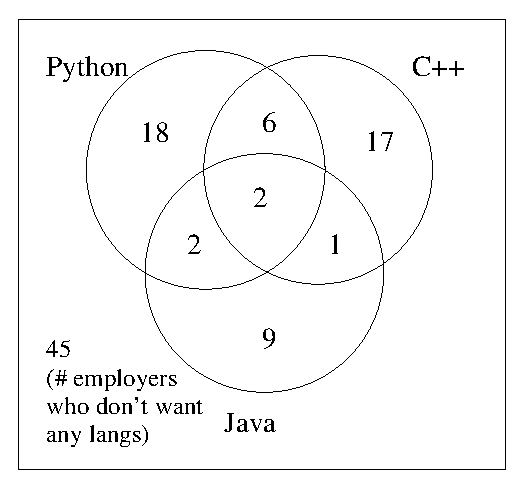
\includegraphics[scale=0.8]{hw12venn}
        
        \item How many employers wanted students to know at least one of the languages?
        
        \textbf{Answer:} 55
        
        \item How many employers wanted students to know Java and Python, but not C++?
        
        \textbf{Answer:} 2
        
        \item How many employers wanted students to know Python and C++, but not Java?
        
        \textbf{Answer:} 6
\end{enumerate}


\end{enumerate}
\end{document}
